 \textbf{GameManager}: è l'elemento principale relativo al controller ed ha varie funzionalità, una di queste è \textit{initializeGame}, per l'inizializzazione del gioco: questo metodo permette di inizializzare la parte di \textit{view}; inoltre permette il caricamento di tutte le sprites utilizzate successivamente nella partita in modo da limitare le lettura da file durante l'esecuzione del gioco; questa operazione è fatta sfruttanto il meccanismo delle Future, quindi al suo completamento verrà mostrata la finestra di gioco.

\textbf{GameLoop}: Come detto prima si è scelto di utilizzare un event-loop per gestire le dinamiche di gioco. Questa classe lo implementa. All'avvio della partita il \textit{GameManager} fa partire un thread separato sul quale viene lanciato un event-loop incaricato di aggiornare la parte view ed, ad ogni ciclo, far compiere uno step alla parte logica. 
Per gestire gli eventi creati dall'utente vengono utilizzate due queue che tengono traccia degli spari e dei movimenti compiuti dall'utente e non ancora processati dall'event-loop. Gli eventi vengono poi recuperati ad ogni step come riportato in figura \ref{checknewMovement}.

\begin{figure}[H]
  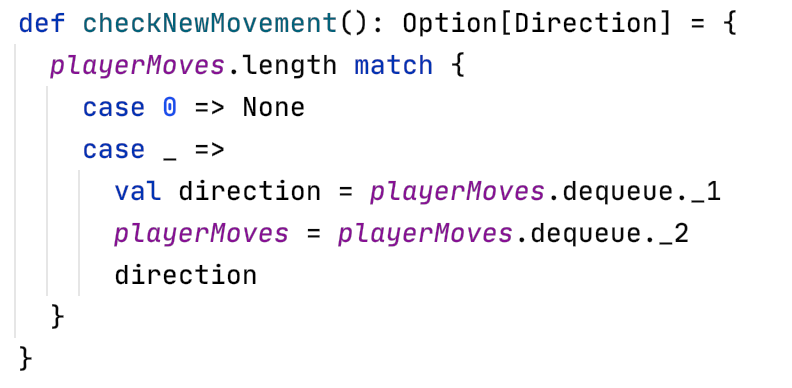
\includegraphics[width=13cm]{report/res/checkNewMovement.png}
  \caption{Recupera un movimento notificato}
  \label{checknewMovement}
\end{figure}
\textbf{ViewObserver}: Interfaccia che rappresenta l'observer della view; è utilizzata per la comunicazione da view a controller, si occupa di notificare le transizioni tra le varie scene; inoltre notifica i \textit{KeyEvent} generati dall'utente e catturati dalla \textit{GameView}. Quando un evento viene notificato viene aggiunto alla relativa coda per essere, successivamente, consumato dal \textit{GameLoop} come riportato in figura \ref{notifyAction}.
\begin{figure}[H]
  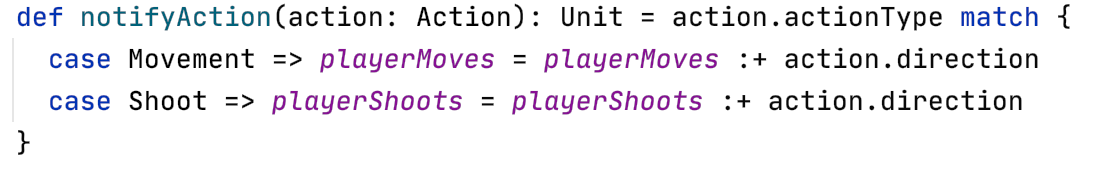
\includegraphics[width=15cm]{report/res/notifyAction.png}
  \caption{Aggiunge l'azione notificata alla relativa Queue}
  \label{notifyAction}
\end{figure}

